
\documentclass[12pt, a4paper, twocolumn]{article}

\usepackage[utf8]{inputenc}
\usepackage{graphicx}
\usepackage[spanish]{babel}
\usepackage[T1]{fontenc}
\usepackage{titling}
\usepackage{titlesec}
\usepackage{fontspec}
\usepackage{wrapfig}
\usepackage{balance}
\usepackage{float}
\usepackage{csquotes}
\usepackage[backend=biber, style=apa]{biblatex}
\usepackage{hyperref}

\usepackage{etoolbox}
\patchcmd{\thebibliography}{\section*}{\section}{}{}

\addbibresource{ref.bib}

\graphicspath{{./Images/}}
\titleformat{\section}{\normalfont\Large\bfseries}{\thetitle. \quad }{0pt}{}[{ \titlerule[0.8pt]}]
\setmainfont{Arial}
%\renewcommand{\familydefault}{\sfdefault}

% Cuales componentes se requieren para armar una computadora desde cero? Describa los componentes y agregue una imagen de cada uno de ellos
% En que orden instalaria los componentes? Puede agregar informacion sobre cada paso, por ejemplo: informacion sobre los tipos de cable, tarjetas, slot de conexion, entre otros
% Cual sistema operativo instalaria?
% Cuales drivers y programas instalaria?
% Presente un presupuesto de los principales componentes de una computadora

\begin{document}
\begin{titlepage}
    \begin{flushleft}
        \textbf{\Large Tarea \#1 Soporte Técnico}
        \newline

        \large Diego Quirós Artiñano \\
        
        \vfill
        
        
\includegraphics[width=0.4\textwidth]{UNA.png}

        Departamento: Escuela de Informática \\
        Curso: EIF202 - Soporte Técnico \\
        Ciclo I \\
        Profesora: Carolina Gómez Fernández \newline

        Fecha: 13 de marzo, 2022
    \end{flushleft}
\end{titlepage}
\section{Componentes de la computadora}
\balance
En esta sección voy a evaluar lo mínimo que se necesita, intentando de que los componentes sea el menor presupuesto posible, el mayor presupuesto al día y lo que idealmente usaría yo.
\subsection{Lista de componentes y presupuesto mínimo}
Para esta lista usé PC PART PICKER (\cite{partpickerminimum}). Para hacer la lista, tuve que verificar si algunos componentes eran necesarios, como la tarjeta gráfica () y la tarjeta de sonido ().
\begin{itemize}
    \item Intel Core 2 Duo E7300 2.66 GHz Dual-Core OEM/Tray Processor  \$11.95
    \item Zalman CNPS80F CPU Cooler                                     \$11.66
    \item MSI G41M4-F Micro ATX LGA775 Motherboard                      \$79.98
    \item Patriot Signature 1GB (1 X 1 GB) DDR2-800 CL6 Memory          \$6.82
    \item Toshiba 320 GB 2.5" 5400RPM Internal Hard Drive               \$13.45
    \item Vision Tek Radeon HD 5450 1 GB Video Card                     \$45.99
    \item BitFenix Nova Mesh SE ATX Mid Tower Case                      \$38.40
    \item Logisys 480 W ATX Power Supply                                \$16.98
    \item Nexus D125L-12BL 36.86 CFM 120 mm Fan                         \$4.99 \\
Aqui estaría completa la computadora (sin poder sonar, ver, usar, accesar al internet y sin pasta térmica)
    \item Acer V206WQL bd 19.5" 1440x900 60 Hz Monitor                  \$87.96
    \item Verbatim 99201 Wired Standard Keyboard                        \$8.94
    \item Verbatim 98618 Mini Travel Mouse Commuter Wired Optical Mouse \$4.99
    \item Total: \$332.11
\end{itemize}
Con esto se tiene para ver y usar y para minimizar costos se le instalaría Linux, aunque aun no se puede usar el internet por falta de adaptadores.
\subsection{Lista de componentes y presupuesto máximo}
Para esta lista usé PC PART PICKER (\cite{partpickermaximum}).
\begin{itemize}
    \item AMD Threadripper 3990X 2.9 GHz 64-Core Processor                          \$5689.00
    \item Corsair H100i RGB PLATINUM 75 CFM Liquid CPU Cooler                       \$379.99
    \item ARCTIC MX-5 Incl. Spatula 20g Thermal Past                                \$99.99
    \item Asus ROG ZENITH II EXTREME ALPHA EATX sTRX4 Motherboard                   \$1609.99
    \item Corsair Dominator Platinum 128 GB (8 x 16 GB) DDR4-3200 CL 16 Memory      \$3879.02
    \item Team QX 15.3 TB 2.5" Solid State Drive                                    \$3299.99
    \item PNY Quadro GV100 32 GB Video Card                                         \$10560.00
    \item Phanteks Eclipse P4005 ATX Mid Tower Case                                 \$1127.58
    \item Corsair AX 1000 W 80+ Titanium Certified Fully Modular ATX Power Supply   \$1199.00
    \item Microsoft Windows 11 Pro OEM 64-bit                                       \$159.99
    \item EVGA NU 24-bit 192 kHz Sound Card                                         \$735.00
    \item StarTech ST1000SPEX42 PCle x4 1 Gbit/s Network Adapter                    \$431.08
    \item Intel 62205 ANHMWDTX1 PCle x1 802.11a/b/g/n Wi-Fi Adapter                 \$149.94
    \item Corsair High Performance 62.74 CFM 120 mm Fan                             \$295.50
    \item Dell UP3216Q 31.5" 3840x2160 60 Hz Monitor                                \$4589.00
    \item Logitech MX 5500 Revolution Wireless Standard Keyboad with Lase Mouse     \$779.00
    \item Logitech G500s Laser Gaming Mouse Wired Laser Mouse                       \$464.50
    \item Logitech THX Z-5300e 280 W 5.1 Channel Speakers                           \$1799.99
    \item Total: \$37249.56 (sin contar el shipping que calcula la página)
\end{itemize}
Aunque la lista dice que el CPU no está con soporte en Windows 11 la página oficial de Microsoft dice lo contrario (\cite{windows11Support}). 
\subsection{Lista de componentes y presupuesto ideal para mi}
\begin{itemize}
    \item 
\end{itemize}
\section{Imágenes de las listas de partes}
\onecolumn
La lista de menor valor: \\
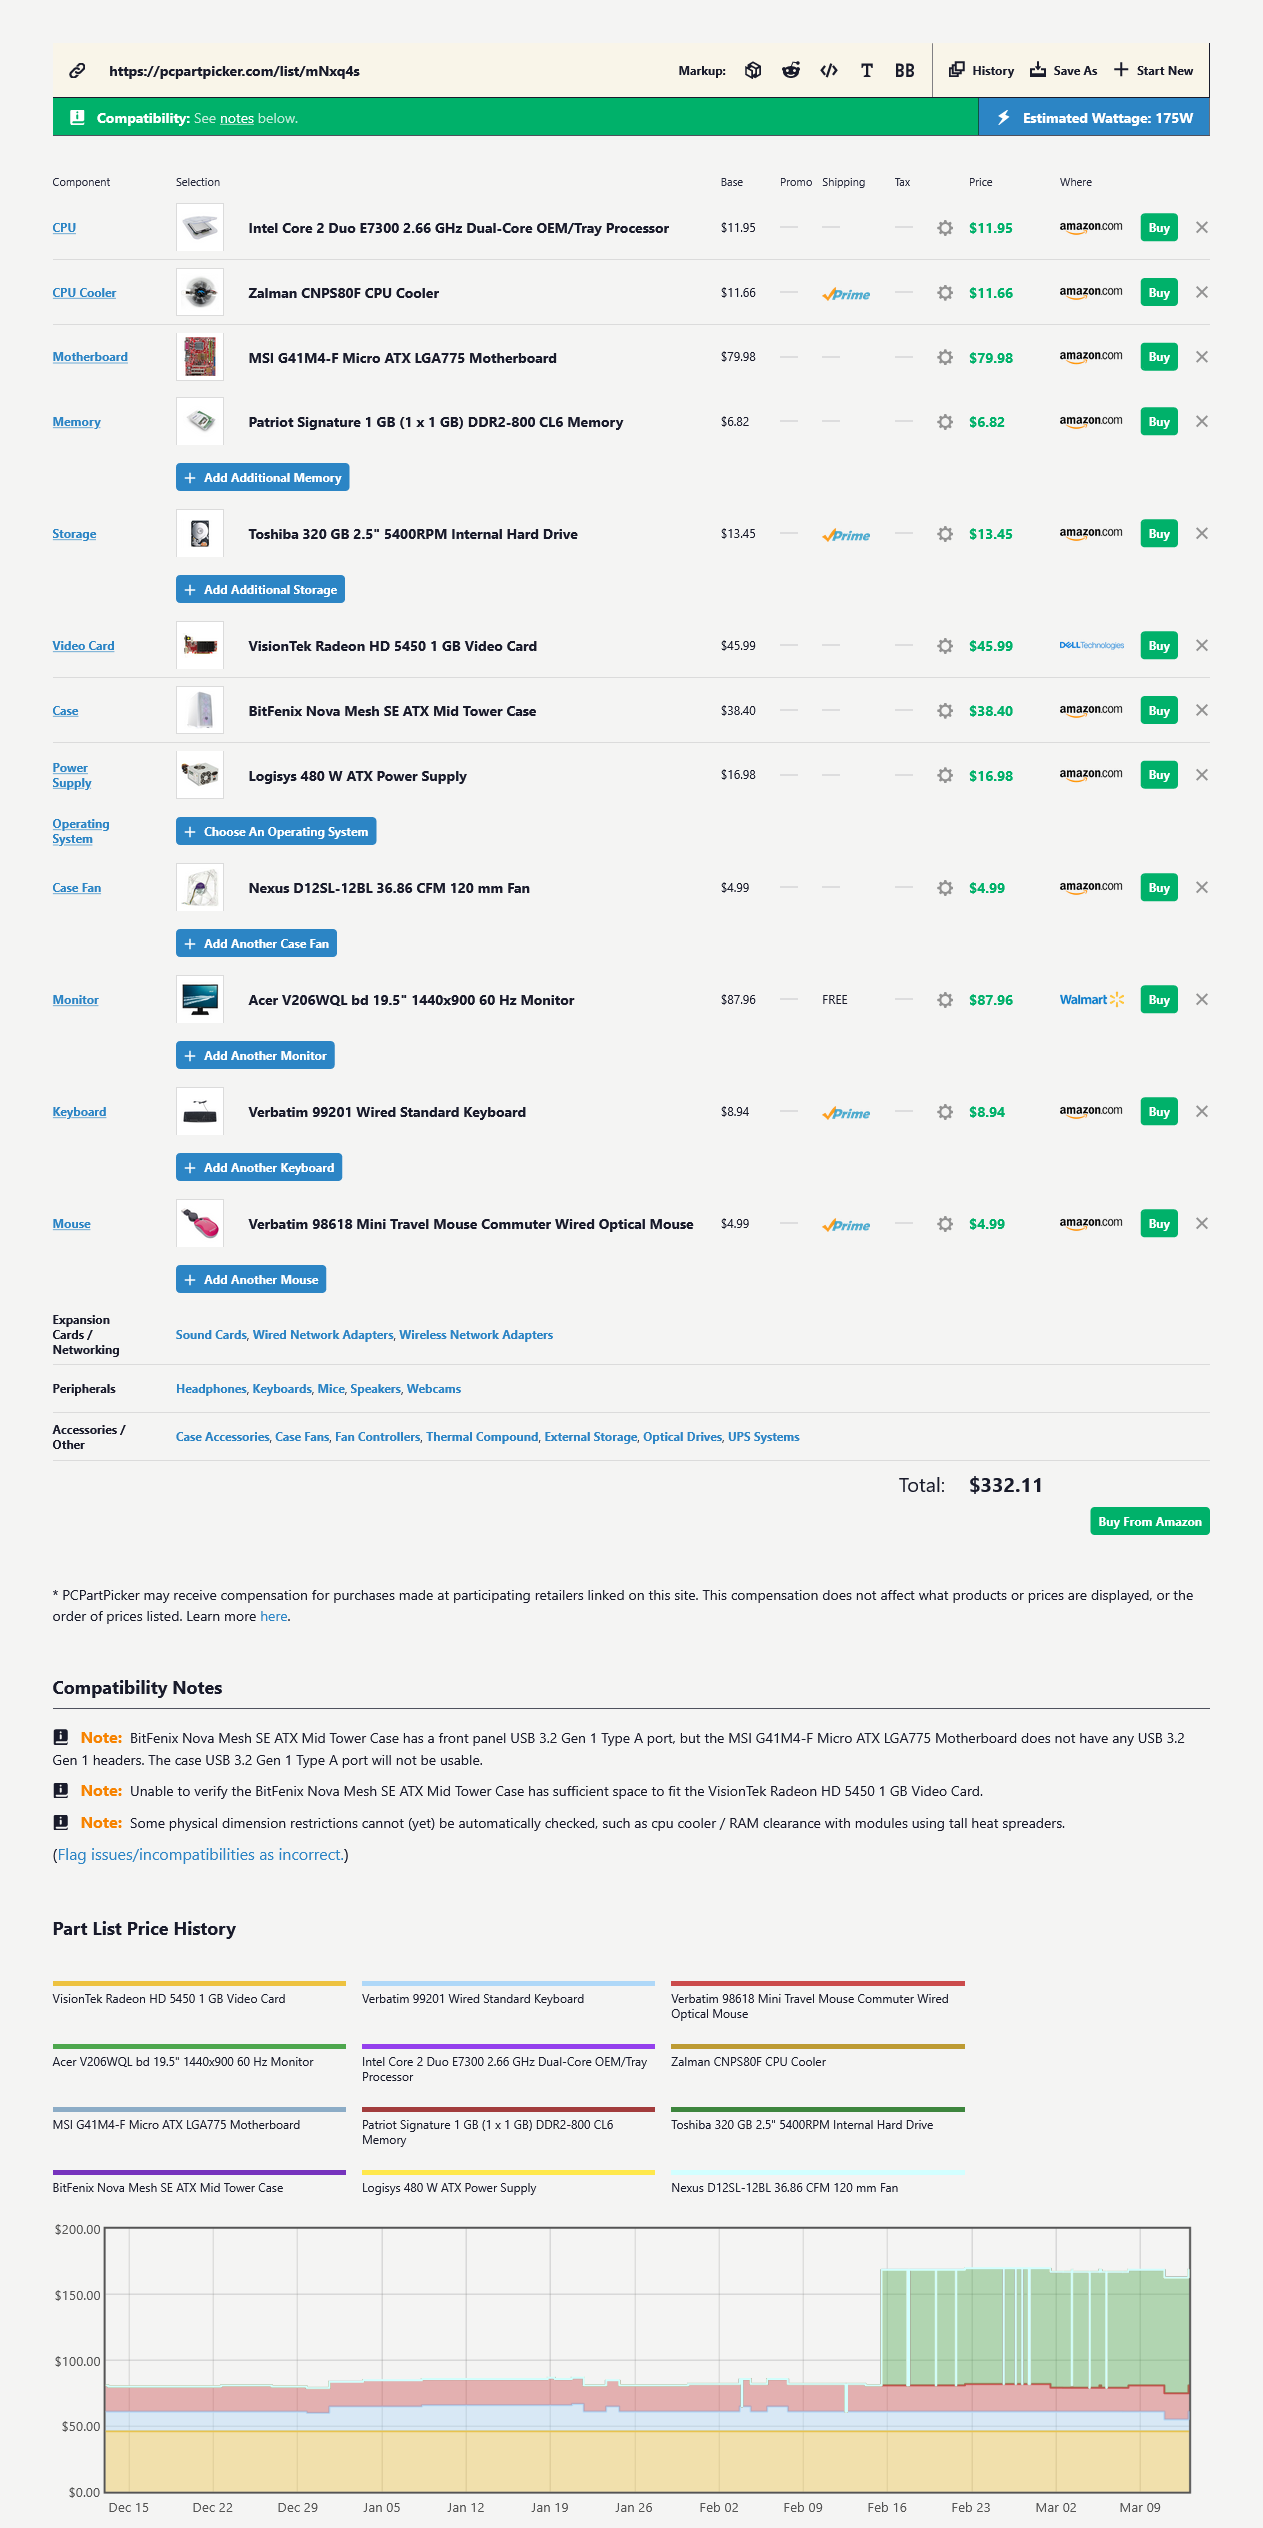
\includegraphics[width=0.6\textwidth]{Minimal.png} \\ \\ \\
La lista de mayor valor: \\
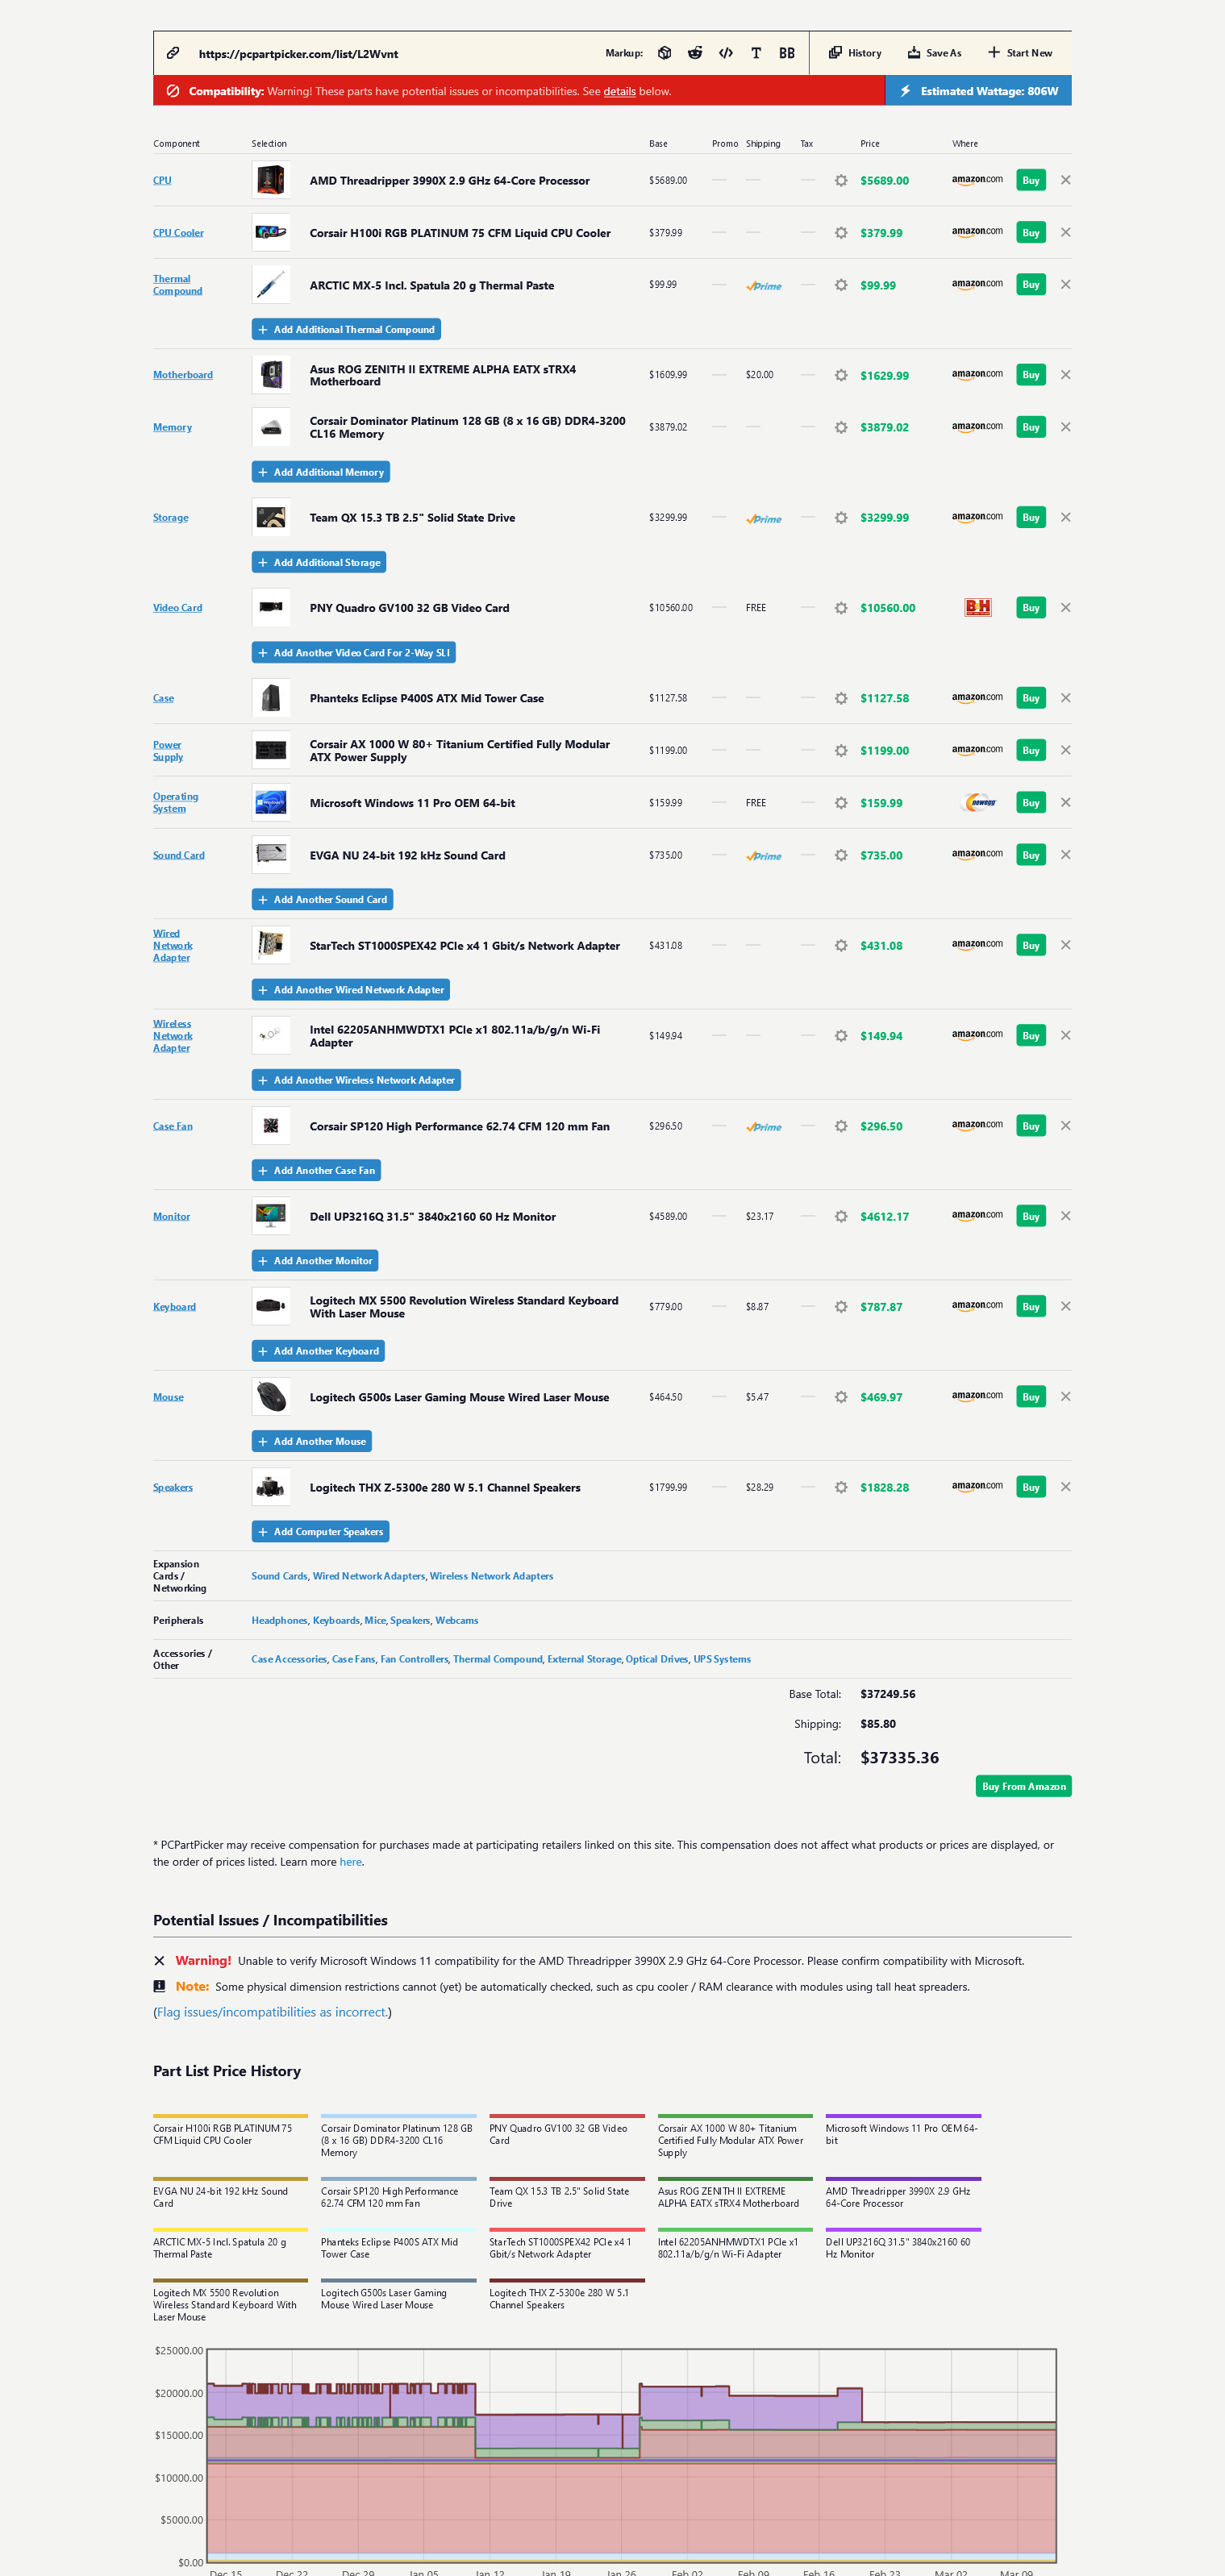
\includegraphics[width=0.6\textwidth]{Maximum.png} \\
\twocolumn
\section{Pasos para armar la computadora}
Para esta parte usé un video de referencia para seguir los pasos de como armar una computadora (\cite{linusTechTips_pcbuilding}).

\newpage
\onecolumn
\printbibliography
% https://www.tomshardware.com/reviews/best-cpus,3986.html
% https://buildredux.com/pages/build-your-pc
% https://www.newegg.com/p/pl?N=100007671&Order=0
% https://electrobot.co.in/blog/do-your-computer-needs-a-graphics-card/
% https://www.cambridgeaudio.com/usa/en/blog/bypass-your-soundcard
\end{document}